%\section{Approach}

\section{Architecture}

\subsection{Overview}


\begin{figure}
\centering
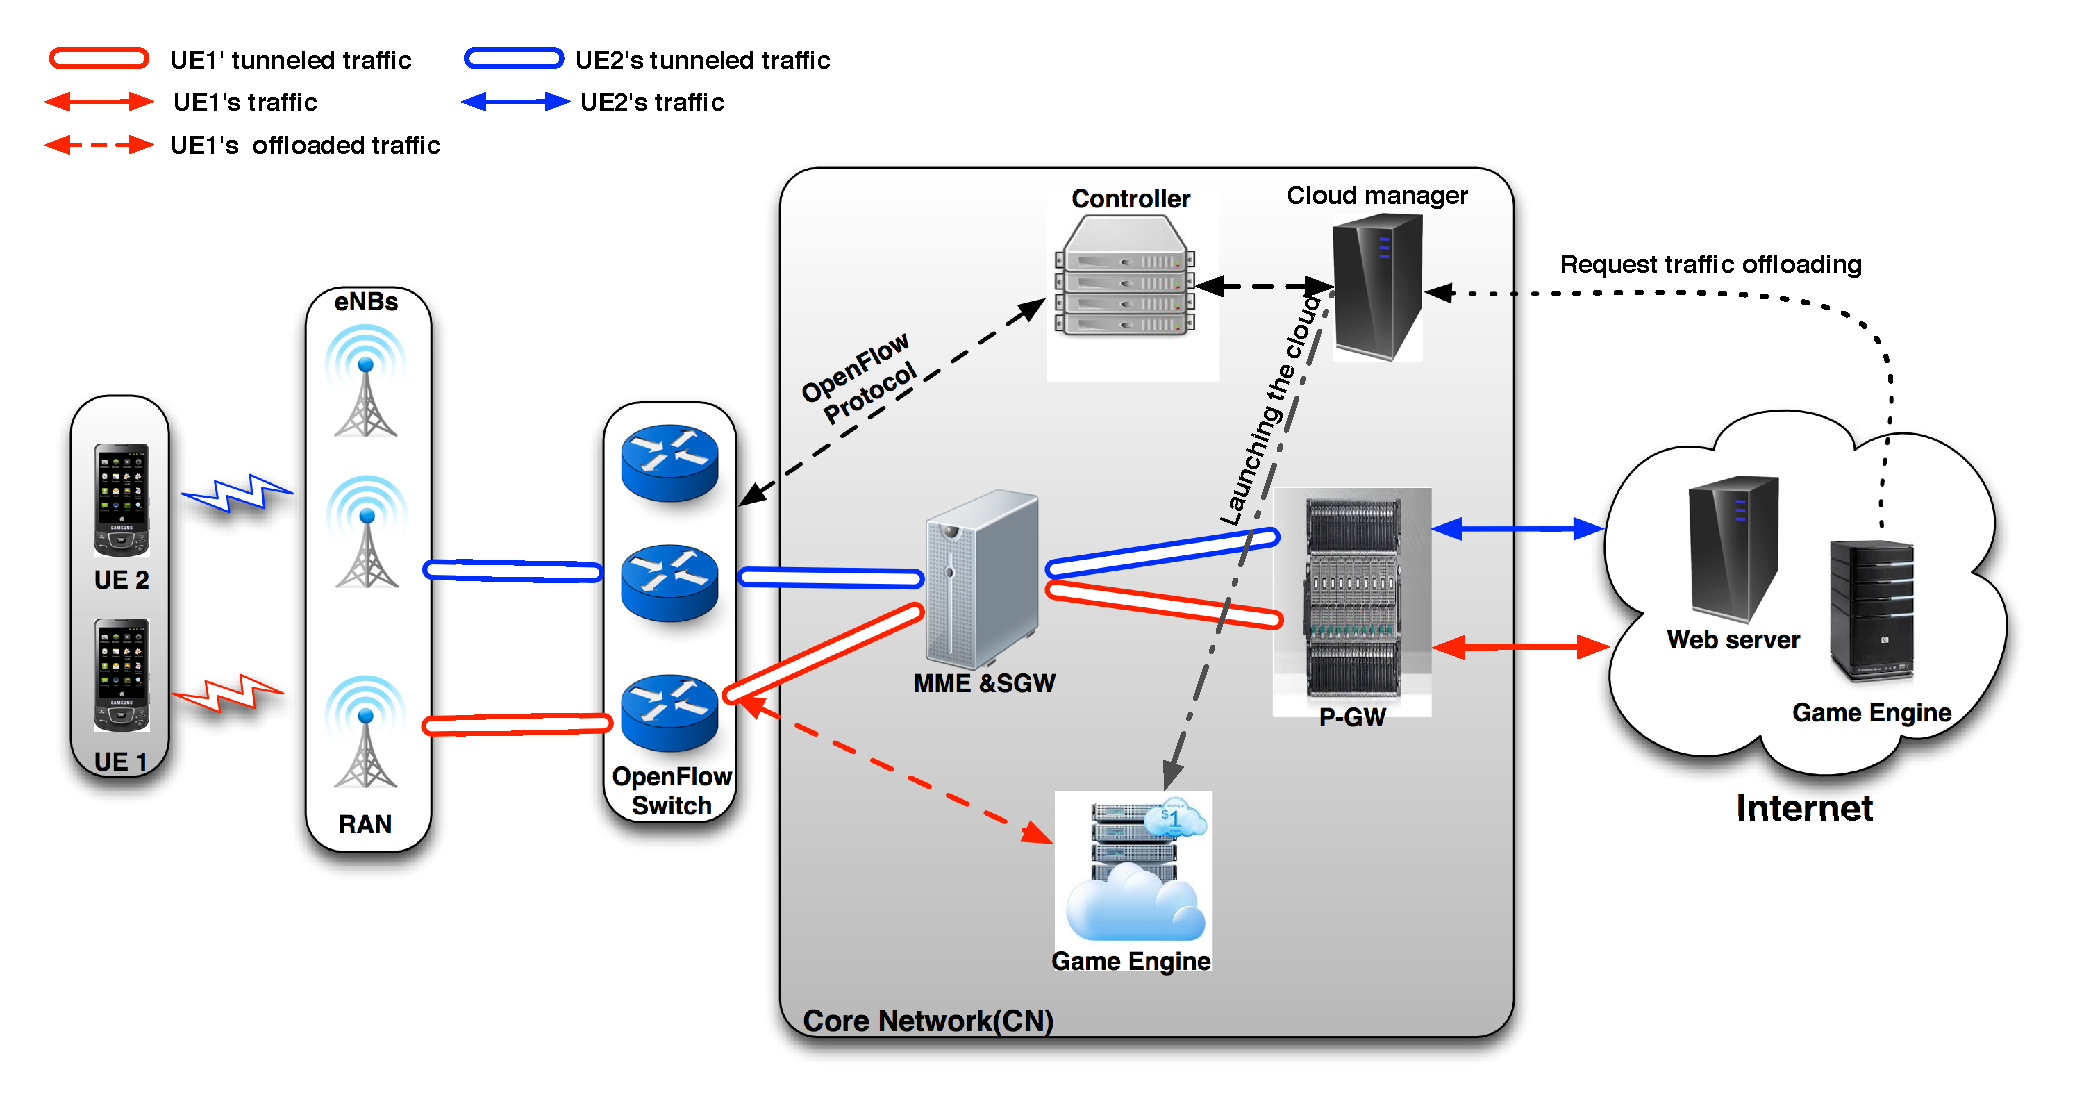
\epsfig{file=./figure/architecture_mobi, height=5.5cm , width=10cm}
\caption{The system architecture}
\label{fig:architecture}
\end{figure}

Our work adds to the current cellular network two main components: a SDN substrate, and a registration and control server. The SDN substrate locates in between the Radio Access Network (RAN) and core network. This substrate consists of Openflow switches (OFSes) that talk to eNodeBs via GTP tunnel. The OFS proactively reroutes offloading traffic at the behest of its controller. The registration server acts as a “brain” of the system. It stores information of traffic that needs offloading (e.g., IP prefix of a game server) and talks to the SDN substrate to realize the offloading functionality.\\

A basic workflow of the system is described as follow: users (e.g., CDN providers) register their services on the central registration center. The central register center then translates these information into SDN rules (e.g., match:actions) and deploys the rules on the SDN substrate. Once these rules are deployed, the SDN substrate is able to reroute registered traffic to appropriate offloading servers while leaving other traffic untouched.


\subsection{Realization}

\subsubsection{Registration server}

The “brain” of the system is the registration server. This server provides an interface that allows users to register for their offloading services. Users specify the properties of their offloading traffic and the QoS associated with the traffic. For example, a game provider registers a list of IP prefixes of game engines that it wants to provide offloading functionality. It is also be able to specify the Quality of Service (QoS) of these offloading traffic if needed. The registration server then translates the high-level registration information into low-level actual SDN rules that are deployable in the SDN substrate. These rules should be able to distinguish and redirect the offloading traffic to offloading servers inside the core (since the SDN substrate is a set of OFSes, routing inside the substrate needs more elaboration).

\subsubsection{SDN substrate}
SDN substrate is a set of OFSes controlled by controller(s). These OFSes forward traffic at the behest of controllers. In contrast with the current architecture, OFSes contact with offloading servers using normal IP links instead of GTP tunnels (as in Firgure ~\ref{fig:architecture}. \\
Current Openflow does not support packet payload matching so OFSes can not forwarding packets based on GTP tunneling information. We propose to modify the OFS implementation to force it do GTP decapsulating before feeding packets into the normal OFS pipe line (packet matching and forwarding based on flow table).\\

\subsubsection{Packet offloading}

When attaches to the network for the first time, 
UE follows a normal attaching process (e.g. 
authentication, bearers establishment, and acquiring 
an IP address from the PGW). After resources are 
allocated, the UE can talk to the server using 
server's IP address. Traffic from UE, however, are 
not fully routed to the Internet as usual but intercepted 
by the OFS, and traffic destined for the registered server 
are rerouted to the local offloading server.
(dotted arrow in Figure ~\ref{fig:architecture}).\\

Packets arrived at the OFS are filtered by OFS's controller.
When arrived at the OFS, packets from UE are GTP 
encapsulated. Since Openflow's data path does not support payload 
matching, GTP packets are sent to OFS's controller for packet 
decapsulation and matching. OFS's controller 
decapsulates the GTP packets and compares their destination IPs 
with the database of registered offloading server's 
IPs. If matched, controller forwards decapsulated packets 
to port that connects to the offloading server. 
In the mean time, controller installs a 
rule for packets in the reversed direction. This 
rule changes the source IP address of the packets 
in the reversed direction as if these packets 
come from the server in the Internet. Therefore, the 
communication is transparent at UE's perspective.\\

















